\section{Introduction}
Large Language Model (LLM)~\cite{gpt,gemini,deepseek,kimi} based search agents~\cite{search-r1,ReSearch,search-o1,manusearch,resp} have emerged as an effective paradigm for complex information-seeking and reasoning tasks~\cite{hotpotqa,2wikimultihop,triviaqa,musique,browsecomp}.
By combining multi-step reasoning with external tool calls, they can iteratively gather evidence and update their intermediate hypotheses.
This enables them to solve problems that standard single-pass LLM generation often fails to handle. 
However, these advantages come with a notable drawback: search agents typically exhibit much higher end-to-end latency.
In complex search-driven agent scenarios, like Deep Research~\cite{openai-deepresearch}, completing a single task can even take up to 30 minutes.


One major source of latency arises from the strict serial dependency in the widely adopted Reason–Action paradigm~\cite{react} of modern LLM search agents.
As illustrated in \Figref{fig:fig1}a, we breakdown the latency of two models (Qwen2.5-32B~\cite{qwen2.5} for Q32, Gemma-3-27B~\cite{Gemma3} for G27) based search agent on three benchmarks~\cite{hotpotqa,2wikimultihop,triviaqa}, both LLM inference and action execution constitute substantial and non-negligible portions of the overall delay.
In each step of the agent workflow, the model must first complete a full inference pass to produce thought and next action; only after the inference finishes can the system execute the action (e.g., issuing a search query via API) and collect the resulting observation.
This rigid ordering forces the two latency-heavy stages to occur strictly one after another, making step-level delay accumulate and ultimately dominate end-to-end task completion time.


\begin{figure}[t]
    \centering
    \begin{subfigure}[b]{0.48\linewidth}
        % \centering
        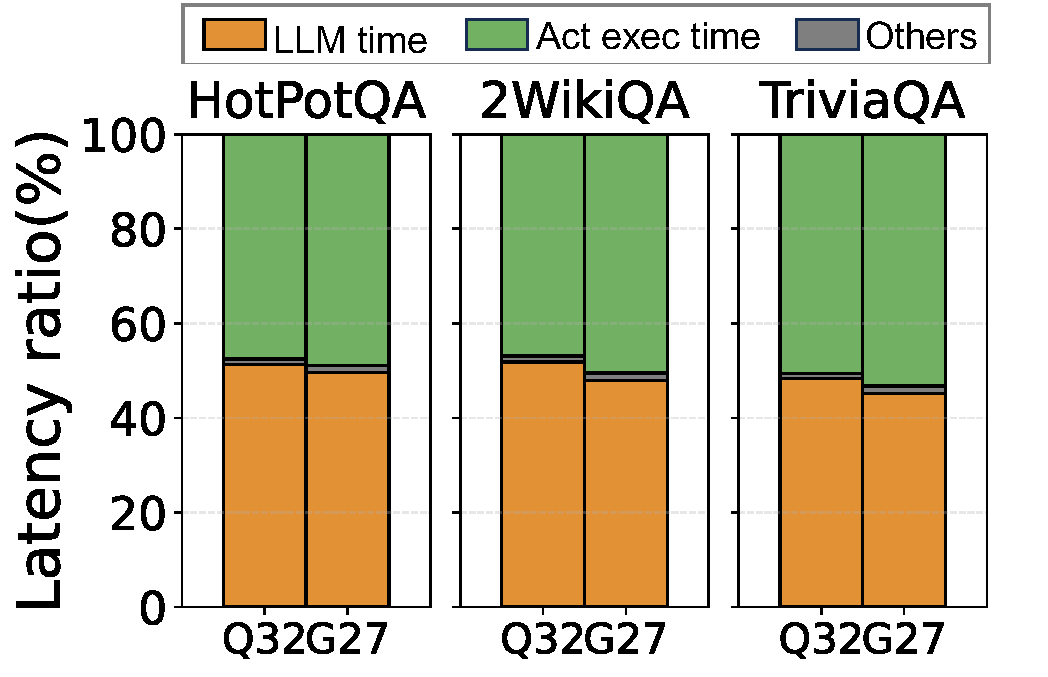
\includegraphics[width=\linewidth]{figures/latency_ori.pdf}
        % \caption{Naive Reason-Action Step.}
        \label{fig:latencr_bd_ori}
    \end{subfigure}
    \hfill
    \begin{subfigure}[b]{0.48\linewidth}
        % \centering
        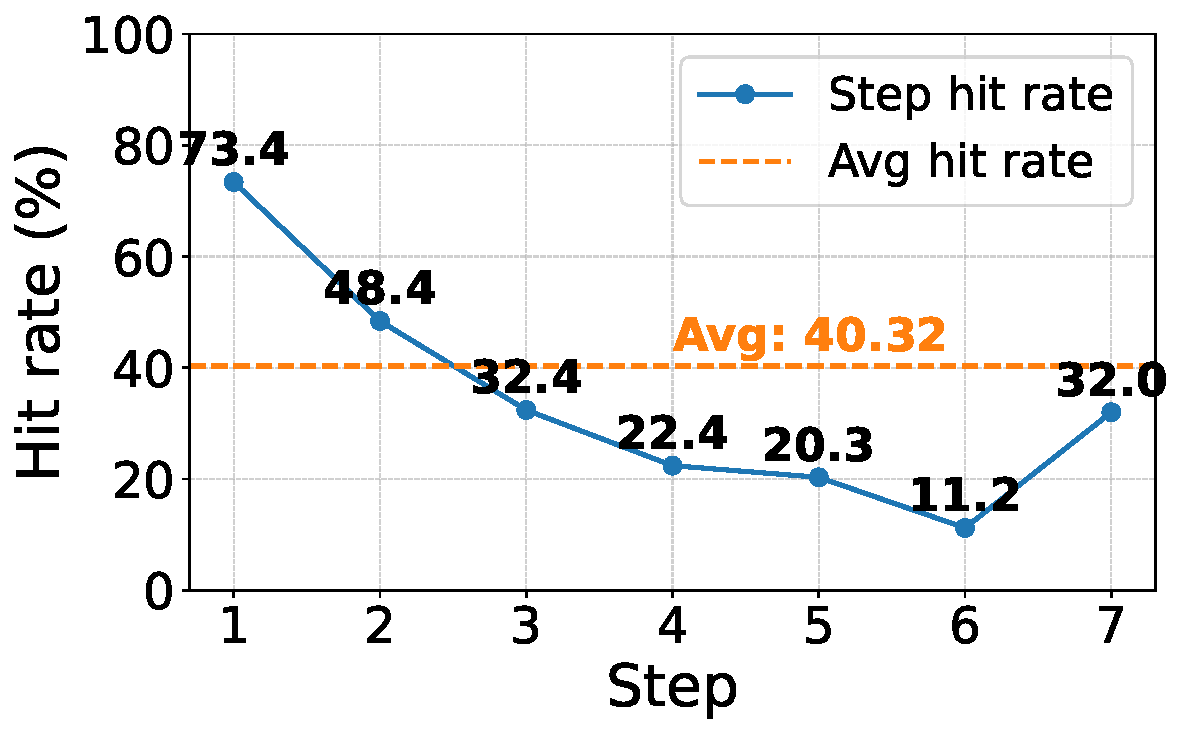
\includegraphics[width=\linewidth]{figures/hit_rate_step.pdf}
        % \caption{Adaptive Speculation Phase Transition.}
        \label{fig:hit_rate_step}
    \end{subfigure}
    \vspace{-15pt}
    \caption{(a) Latency breakdown ratio of search agent tasks. (b) Speculative action hit rate across search agent steps.}
    \label{fig:fig1}
    \vspace{-15pt}
\end{figure}


To address the long latency stemming from the strict serial dependency, a natural direction is to draw on speculation.
In domains such as branch prediction~\cite{branchpredict} and speculative decoding~\cite{speculativedecoding,speculativesampling,eagle}, a predict-verify paradigm enables future work to be carried out ahead of time and later validated, effectively reducing end-to-end latency.
Following this idea, we propose that LLM search agents can adopt it in the \textbf{action level}: 
Agent can generate actions directly without reasoning tokens, and execute these actions in parallel with the original reasoning progress.

However, the predict-verify paradigm also comes with fundamental limitations: 
it preserves the full original computation while adding speculative work on top, meaning only correct predictions yield speedups, and the additional inference required for speculation introduces non-negligible overhead.

Given these limitations of the predict-verify paradigm, we demonstrate that \textbf{not all speculative actions require verification} in search agents.
As illustrated in \Figref{fig:fig1}b, speculative actions achieve a 73.4\% hit rate in the first step, far exceeding the overall average of 40\%.
Equally important, early-step mistakes are low-risk: 
These actions serve mainly to gather information, and an incorrect speculative action often still task-relevant and sometimes even providing useful auxiliary evidence, rather than causing irreversible deviations in the agent's reasoning trajectory or corrupting internal context~\cite{ircot}.
Thus, omitting verification in early steps offers substantial latency savings by eliminating inference overhead while incurring only minimal, recoverable cost when speculation is wrong.



To reduce the long latency of search agents based on our observations, we propose \system, a holistic algorithm-system co-designed framework that leverages action speculation in search agents that both shorten LLM inference time and overlap tool-execution time. 


At the algorithm level, action speculation presents a tension between efficiency and accuracy.
Aggressive speculation without verification can effectively reduce inference latency but risks producing unreasonable actions, whereas speculation with reasoning-based verification preserves accuracy but adds inference overhead.
Thus, an effective agent must adaptively choose between these two modes to minimize latency without harming answer quality (\Secref{sec:algo}).

At the system level, speculation introduces additional inference requests and increases heterogeneity in the workload, as speculative requests produce far shorter outputs than full reasoning ones.
This higher and more uneven load can delay ongoing reasoning and becomes especially problematic under high concurrency~\cite{turbospec}.
Moreover, speculative requests must finish early enough to precede their corresponding reasoning requests; otherwise, they fail to create any overlap for latency reduction.
To address these challenges, \system employs a two-level scheduling strategy (\Secref{sec:system}): an intra-speculation scheduling that adaptively controls and selects speculative launches based on current engine load; and an inter-request scheduling that prioritizes short speculative requests using an Short-Job-First (SJF)~\cite{osconcept} inspired policy to ensure timely completion and effective parallelism.


In summary, this work makes the following contributions:

\begin{itemize}[leftmargin=*]
    \item We introduce a \textbf{new speculation paradigm} for multi-step search agents that goes beyond traditional predict-verify schemes.
    This features a two-phase design that jointly reduces LLM inference latency and overlaps external action-execution latency while preserving answer accuracy.
    \item We design a two-level \textbf{speculation-aware scheduling} architecture that coordinates speculative and other inference requests under real-world inference engine constraints. 
    This system-level co-design ensures that speculation delivers actual latency reduction even in concurrent serving environments.
    \item We build a full system implementation of \system and deployed on three types of GPU platforms (including NVIDIA RTX 3090, A100, A800). We conduct extensive evaluations across diverse models, benchmarks, and deployment scenarios.
    
\end{itemize}
Experiments demonstrate that \system significantly reduces end-to-end latency, achieving up to $1.65\times$ end-to-end speedup while maintaining comparable answer quality, enabling practical deployment of search agents in both cloud and edge scenarios.